\documentclass[serif]{beamer}
\usepackage[UTF8]{ctexcap}
\usepackage{amsmath,mathtools,hyperref,caption,wrapfig,enumitem}
\usetheme{Antibes}
\usecolortheme{beaver}

\newtheorem{thm}{定理}
\renewcommand\proofname{\heiti 证明}

\usepackage{pgfplots}
\pgfplotsset{compat=1.15}
\usepackage{mathrsfs}
\usetikzlibrary{arrows}

\title{\textbf{\heiti 勾股定理及其证明}}
\author{\kaishu 程昊一}
\date{}

\begin{document}

\setlength\abovedisplayskip{0.2cm}
\setlength\belowdisplayskip{0.2cm}

\begin{frame}
	\maketitle
\end{frame}

\section{\heiti 勾股定理}

\begin{frame}{\heiti 勾股定理}
	\textbf{勾股定理}: 在直角三角形中, 两直角边的平方和等于斜边的平方.
	
\end{frame}

\section{\heiti 勾股定理的若干证明}
\subsection{\kaishu 1. 毕达哥拉斯证}

\begin{frame}{\heiti 勾股定理的若干证明}

	\begin{columns}
		\column{6.5cm}
		\textbf{1. 毕达哥拉斯证法}\par
		如图, $\mathrm{Rt}\triangle ABC$中, $\angle C=90^\circ$, 以$AB$, $BC$, $CA$为边向外作正方形$ABDE$, $BCFG$, $CAHK$.过$C$作$CP\perp DE$于$P$. 连接$CE$, $CD$, $BH$, $AG$.不难知道
		\[\triangle HAB\cong\triangle CAE, \triangle GBA\cong\triangle CBD.\]
		$\therefore$
		\vspace*{-0.65cm}
		\begin{align*}
		 	&S_{\text{正方形}CAHK}+S_{\text{正方形}BCFG}\\
			=&2\left(S_{\triangle HAB}+S_{\triangle GBA}\right)\\
			=&2\left(S_{\triangle CAE}+S_{\triangle CBD}\right)\\
			=&S_{\text{正方形}ABDE}.
		\end{align*}
		
		\column{4cm}
		\begin{figure}
			\centering
			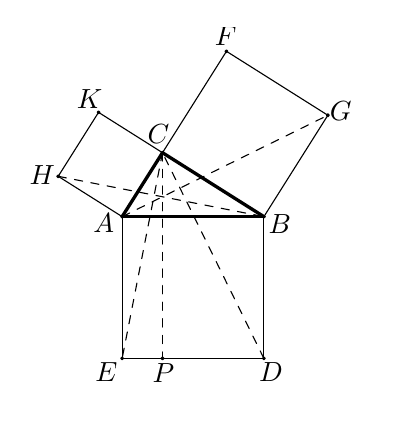
\begin{tikzpicture}[line cap=round,line join=round,>=triangle 45,x=0.6cm,y=0.6cm]
				\clip(-2.,-4.) rectangle (5.5,4.);
				\draw [line width=1.2pt] (0.8538252410154988,1.353683190724965)-- (0.,0.);
				\draw [line width=1.2pt] (0.8538252410154988,1.353683190724965)-- (3.,0.);
				\draw [line width=1.2pt] (3.,0.)-- (0.,0.);
				\draw [line width=0.4pt] (-0.49985794970946607,2.2075084317404636)-- (0.8538252410154988,1.353683190724965);
				\draw [line width=0.4pt] (0.,0.)-- (-1.353683190724965,0.8538252410154988);
				\draw [line width=0.4pt] (-1.353683190724965,0.8538252410154988)-- (-0.49985794970946607,2.2075084317404636);
				\draw [line width=0.4pt] (0.8538252410154988,1.353683190724965)-- (2.2075084317404636,3.499857949709466);
				\draw [line width=0.4pt] (2.2075084317404636,3.499857949709466)-- (4.353683190724965,2.1461747589845013);
				\draw [line width=0.4pt] (4.353683190724965,2.1461747589845013)-- (3.,0.);
				\draw [line width=0.4pt] (3.,0.)-- (3.,-3.);
				\draw [line width=0.4pt] (3.,-3.)-- (0.,-3.);
				\draw [line width=0.4pt] (0.,-3.)-- (0.,0.);
				\draw [line width=0.4pt,dash pattern=on 3pt off 3pt] (0.8538252410154988,1.353683190724965)-- (0.8538252410154988,-3.);
				\draw [line width=0.4pt,dash pattern=on 3pt off 3pt] (0.8538252410154988,1.353683190724965)-- (0.,-3.);
				\draw [line width=0.4pt,dash pattern=on 3pt off 3pt] (3.,-3.)-- (0.8538252410154988,1.353683190724965);
				\draw [line width=0.4pt,dash pattern=on 3pt off 3pt] (-1.353683190724965,0.8538252410154988)-- (3.,0.);
				\draw [line width=0.4pt,dash pattern=on 3pt off 3pt] (0.,0.)-- (4.353683190724965,2.1461747589845013);
				\draw [fill=black] (0.,0.) circle (0.5pt);
				\draw[color=black] (-0.3908286130118098,-0.1357144726562471) node {$A$};
				\draw [fill=black] (3.,0.) circle (0.5pt);
				\draw[color=black] (3.338367670170288,-0.1475531910155553) node {$B$};
				\draw [fill=black] (0.8538252410154988,1.353683190724965) circle (0.5pt);
				\draw[color=black] (0.7693657862003984,1.7584804648330714) node {$C$};
				\draw [fill=black] (0.,-3.) circle (0.5pt);
				\draw[color=black] (-0.33163502121526856,-3.296652274591547) node {$E$};
				\draw [fill=black] (3.,-3.) circle (0.5pt);
				\draw[color=black] (3.148948176421356,-3.287458682795006) node {$D$};
				\draw [fill=black] (2.2075084317404636,3.499857949709466) circle (0.5pt);
				\draw[color=black] (2.190011989317388,3.8184174593527054) node {$F$};
				\draw [fill=black] (-1.353683190724965,0.8538252410154988) circle (0.5pt);
				\draw[color=black] (-1.693087632535717,0.8824153062442616) node {$H$};
				\draw [fill=black] (4.353683190724965,2.1461747589845013) circle (0.5pt);
				\draw[color=black] (4.628787971334887,2.2320291992054013) node {$G$};
				\draw [fill=black] (-0.49985794970946607,2.2075084317404636) circle (0.5pt);
				\draw[color=black] (-0.686796571994516,2.4806422847508744) node {$K$};
				\draw [fill=black] (0.8538252410154988,-3.) circle (0.5pt);
				\draw[color=black] (0.8759142514341727,-3.3084909929508552) node {$P$};
			\end{tikzpicture}
		\end{figure}
	\end{columns}
\end{frame}

\subsection{\kaishu 2. 射影定理证法}

\begin{frame}
	\begin{columns}
		\column{7cm}
		\textbf{2. 射影定理证法}\par
		如图, $\mathrm{Rt}\triangle ABC$中, $\angle C=90^\circ$, 作$AB$边上的高$CD$. 则由射影定理有
		\[AC^2=AD\cdot AB, BC^2=BD\cdot BA.\]
		两式相加得到
		\[AC^2+BC^2=AB\cdot(AD+DB)=AB^2.\]
		\column{3.5cm}
		\begin{figure}
			\centering
			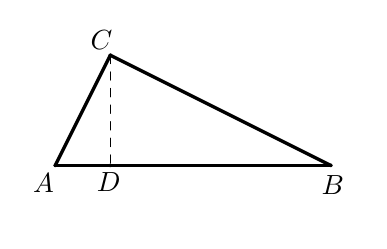
\begin{tikzpicture}[line cap=round,line join=round,>=triangle 45,x=0.7cm,y=0.7cm]
				\clip(-0.5,-1) rectangle (5.5,2.5);
				\draw [line width=1.2pt] (1.,2.)-- (0.,0.);
				\draw [line width=1.2pt] (5.,0.)-- (0.,0.);
				\draw [line width=1.2pt] (5.,0.)-- (1.,2.);
				\draw [line width=0.4pt,dash pattern=on 3pt off 3pt] (1.,2.)-- (1.,0.);
				\draw [fill=black] (0.,0.) circle (0.5pt);
				\draw[color=black] (-0.21428288916969776,-0.32774426113223408) node {$A$};
				\draw [fill=black] (5.,0.) circle (0.5pt);
				\draw[color=black] (5.034886238192234,-0.3505338639792644) node {$B$};
				\draw [fill=black] (1.,2.) circle (0.5pt);
				\draw[color=black] (0.8384350951638765,2.278424416429941) node {$C$};
				\draw [fill=black] (1.,0.) circle (0.5pt);
				\draw[color=black] (0.9682222439173308,-0.30495465828520375) node {$D$};
			\end{tikzpicture}
		\end{figure}
	\end{columns}
\end{frame}

\subsection{\kaishu 3. 张景中证法}

\begin{frame}
	\begin{columns}
		\column{7cm}
		\textbf{3. 张景中证法(算两次原理)}\par
		如图, 做等腰$\mathrm{Rt}\triangle ACD$与等腰$\mathrm{Rt}\triangle BCE$, 易知$AB\perp DE$且$DE=AB$.
		\[\therefore S_{\text{四边形}ADBE}=\frac{1}{2}AB\cdot DE=\frac{1}{2} AB^2.\]
		另一方面, 
		\[S_{\text{四边形}ADBE}=S_{\triangle ADC}+S_{\triangle BCE}\]\[=\frac12\left(AC^2+BC^2\right).\]
		由此立得$AC^2+BC^2=AB^2$.
		\column{3.5cm}
		\begin{figure}
			\centering
			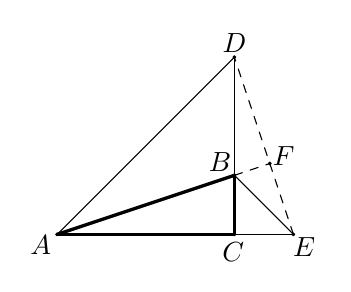
\begin{tikzpicture}[line cap=round,line join=round,>=triangle 45,x=0.75cm,y=0.75cm]
				\clip(-0.5,-0.5) rectangle (4.5,3.5);
				\draw [line width=0.4pt] (3.,1.)-- (4.,0.);
				\draw [line width=0.4pt] (0.,0.)-- (3.,3.);
				\draw [line width=1.2pt] (3.,1.)-- (0.,0.);
				\draw [line width=0.4pt,dash pattern=on 3pt off 3pt] (4.,0.)-- (3.,3.);
				\draw [line width=0.4pt,dash pattern=on 3pt off 3pt] (3.,1.)-- (3.6,1.2);
				\draw [line width=1.2pt] (0.,0.)-- (3.,0.);
				\draw [line width=0.4pt] (3.,0.)-- (4.,0.);
				\draw [line width=0.4pt] (3.,1.)-- (3.,3.);
				\draw [line width=1.2pt] (3.,1.)-- (3.,0.);
				\draw [fill=black] (3.,0.) circle (0.5pt);
				\draw[color=black] (2.981313146613087,-0.30339089409177188) node {$C$};
				\draw [fill=black] (0.,0.) circle (0.5pt);
				\draw[color=black] (-0.27948909174553876,-0.18221685358295042) node {$A$};
				\draw [fill=black] (3.,1.) circle (0.5pt);
				\draw[color=black] (2.7589857212704536,1.2258568402536771) node {$B$};
				\draw [fill=black] (3.,3.) circle (0.5pt);
				\draw[color=black] (3.0024871871219094,3.2479777088461277) node {$D$};
				\draw [fill=black] (4.,0.) circle (0.5pt);
				\draw[color=black] (4.18293994548875,-0.21397791434618266) node {$E$};
				\draw [fill=black] (3.6,1.2) circle (0.5pt);
				\draw[color=black] (3.8335682770931823,1.3211400225433738) node {$F$};
			\end{tikzpicture}
		\end{figure}
	\end{columns}
\end{frame}

\subsection{\kaishu 4. 分块法}

\begin{frame}
	\begin{columns}
		\column{11.5cm}
		\textbf{4. 分块法}\par
		下面给出几种构造方法供大家欣赏. 其主要思路就是通过分块证明以两直角边为边的正方形的面积之和等于以斜边为边的正方形的面积. 下图标为相同编号的块相互全等.
	\end{columns}
	\begin{figure}
		\centering
		\begin{minipage}{0.48\textwidth}
			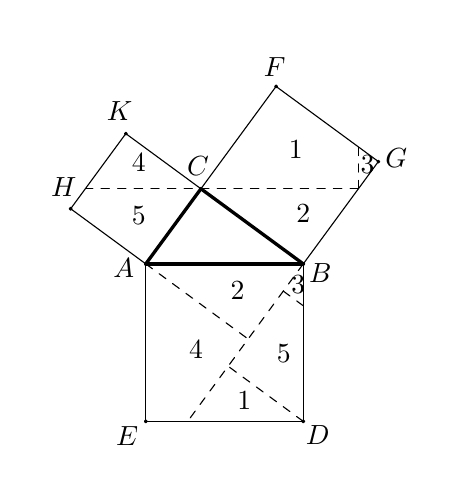
\begin{tikzpicture}[line cap=round,line join=round,>=triangle 45,x=1.0cm,y=1.0cm]
				\clip(-1.5,-2.5) rectangle (3.5,3);
				\draw [line width=1.2pt] (0.7003491424229839,0.9540489314250914)-- (0.,0.);
				\draw [line width=1.2pt] (0.,0.)-- (2.,0.);
				\draw [line width=1.2pt] (2.,0.)-- (0.7003491424229839,0.9540489314250914);
				\draw [line width=0.4pt] (0.7003491424229839,0.9540489314250914)-- (1.6543980738480752,2.2536997890021078);
				\draw [line width=0.4pt] (1.6543980738480752,2.2536997890021078)-- (2.9540489314250915,1.2996508575770163);
				\draw [line width=0.4pt] (2.9540489314250915,1.2996508575770163)-- (2.,0.);
				\draw [line width=0.4pt] (2.,0.)-- (2.,-2.);
				\draw [line width=0.4pt] (2.,-2.)-- (0.,-2.);
				\draw [line width=0.4pt] (0.,-2.)-- (0.,0.);
				\draw [line width=0.4pt] (0.,0.)-- (-0.9540489314250914,0.7003491424229839);
				\draw [line width=0.4pt] (-0.9540489314250914,0.7003491424229839)-- (-0.25369978900210755,1.6543980738480752);
				\draw [line width=0.4pt] (-0.25369978900210755,1.6543980738480752)-- (0.7003491424229839,0.9540489314250914);
				\draw [line width=0.4pt,dash pattern=on 3pt off 3pt] (2.700349142422984,0.9540489314250914)-- (2.700349142422984,1.4858870387706944);
				\draw [line width=0.4pt,dash pattern=on 3pt off 3pt] (2.700349142422984,0.9540489314250914)-- (-0.7678127502314135,0.9540489314250914);
				\draw [line width=0.4pt,dash pattern=on 3pt off 3pt] (2.,0.)-- (0.5318381073456024,-2.);
				\draw [line width=0.4pt,dash pattern=on 3pt off 3pt] (2.,-2.)-- (1.0459510685749085,-1.2996508575770163);
				\draw [line width=0.4pt,dash pattern=on 3pt off 3pt] (0.,0.)-- (1.2996508575770163,-0.9540489314250914);
				\draw [line width=0.4pt,dash pattern=on 3pt off 3pt] (1.7463002109978925,-0.3456019261519248)-- (2.,-0.5318381073456024);
				\draw (1.6918808942577652,1.6830415036331245) node[anchor=north west] {$1$};
				\draw (1.0381234727679456,-1.5000069255877952) node[anchor=north west] {$1$};
				\draw (1.78833690726446,0.8792413952440034) node[anchor=north west] {$2$};
				\draw (0.9523847945397725,-0.10675340437998532) node[anchor=north west] {$2$};
				\draw (2.6028543504321044,1.500846812398257) node[anchor=north west] {$3$};
				\draw (1.7240328985933302,-0.02101472615181239) node[anchor=north west] {$3$};
				\draw (-0.3015433745472587,1.5222814819553003) node[anchor=north west] {$4$};
				\draw (0.4272353903922124,-0.8569668388764984) node[anchor=north west] {$4$};
				\draw (1.5418382073584624,-0.8998361779905849) node[anchor=north west] {$5$};
				\draw (-0.3015433745472587,0.8470893909084385) node[anchor=north west] {$5$};\draw [fill=black] (0.,0.) circle (0.5pt);
				\draw[color=black] (-0.28010870499021545,-0.05852539787663806) node {$A$};
				\draw [fill=black] (2.,0.) circle (0.5pt);
				\draw[color=black] (2.217030298405325,-0.11211207176924613) node {$B$};
				\draw [fill=black] (0.7003491424229839,0.9540489314250914) circle (0.5pt);
				\draw[color=black] (0.6630167555196883,1.2382721103244774) node {$C$};
				\draw [fill=black] (0.,-2.) circle (0.5pt);
				\draw[color=black] (-0.23723936587612887,-2.180557684023918) node {$E$};
				\draw [fill=black] (-0.9540489314250914,0.7003491424229839) circle (0.5pt);
				\draw[color=black] (-1.0410394742652513,0.9810560756399587) node {$H$};
				\draw [fill=black] (1.6543980738480752,2.2536997890021078) circle (0.5pt);
				\draw[color=black] (1.6382942203651571,2.5029176141900282) node {$F$};
				\draw [fill=black] (2.,-2.) circle (0.5pt);
				\draw[color=black] (2.1848782940697604,-2.1698403492453964) node {$D$};
				\draw [fill=black] (2.9540489314250915,1.2996508575770163) circle (0.5pt);
				\draw[color=black] (3.1815904284722722,1.3454454581096935) node {$G$};
				\draw [fill=black] (-0.25369978900210755,1.6543980738480752) circle (0.5pt);
				\draw[color=black] (-0.33369537888282363,1.9456162057069042) node {$K$};
			\end{tikzpicture}
		\end{minipage}
		\begin{minipage}{0.48\textwidth}
			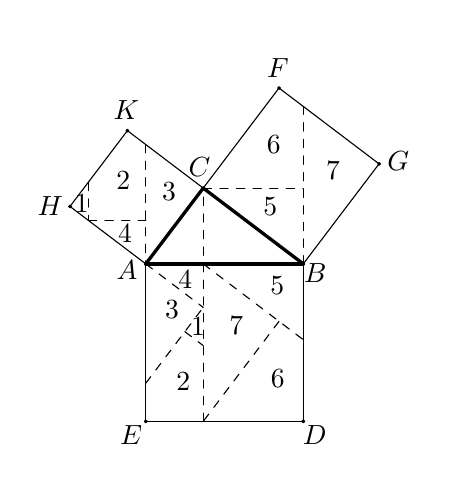
\begin{tikzpicture}[line cap=round,line join=round,>=triangle 45,x=1.0cm,y=1.0cm]
				\clip(-1.5,-2.5) rectangle (3.5,3.);
				\draw [line width=1.2pt] (0.,0.)-- (0.7294706649229483,0.9627117319648537);
				\draw [line width=1.2pt] (0.7294706649229483,0.9627117319648537)-- (2.,0.);
				\draw [line width=1.2pt] (2.,0.)-- (0.,0.);
				\draw [line width=0.4pt] (-0.9627117319648537,0.7294706649229483)-- (0.,0.);
				\draw [line width=0.4pt] (-0.9627117319648537,0.7294706649229483)-- (-0.2332410670419054,1.692182396887802);
				\draw [line width=0.4pt] (-0.2332410670419054,1.692182396887802)-- (0.7294706649229483,0.9627117319648537);
				\draw [line width=0.4pt] (0.7294706649229483,0.9627117319648537)-- (1.692182396887802,2.2332410670419054);
				\draw [line width=0.4pt] (1.692182396887802,2.2332410670419054)-- (2.9627117319648537,1.2705293350770517);
				\draw [line width=0.4pt] (2.9627117319648537,1.2705293350770517)-- (2.,0.);
				\draw [line width=0.4pt] (2.,0.)-- (2.,-2.);
				\draw [line width=0.4pt] (2.,-2.)-- (0.,-2.);
				\draw [line width=0.4pt] (0.,-2.)-- (0.,0.);
				\draw [line width=0.4pt,dash pattern=on 3pt off 3pt] (0.7294706649229483,-2.)-- (0.7294706649229483,0.9627117319648537);
				\draw [line width=0.4pt,dash pattern=on 3pt off 3pt] (0.7294706649229482,0.)-- (2.,-0.9627117319648538);
				\draw [line width=0.4pt,dash pattern=on 3pt off 3pt] (1.6921823968878016,-0.7294706649229484)-- (0.7294706649229483,-2.);
				\draw [line width=0.4pt,dash pattern=on 3pt off 3pt] (0.,0.)-- (0.7294706649229482,-0.5527380973088162);
				\draw [line width=0.4pt,dash pattern=on 3pt off 3pt] (0.,-1.5154498292736696)-- (0.7294706649229482,-0.5527380973088162);
				\draw [line width=0.4pt,dash pattern=on 3pt off 3pt] (0.,1.51544982927367)-- (0.,0.);
				\draw [line width=0.4pt,dash pattern=on 3pt off 3pt] (2.,0.)-- (2.,2.);
				\draw [line width=0.4pt,dash pattern=on 3pt off 3pt] (0.7294706649229483,0.9627117319648537)-- (2.,0.9627117319648537);
				\draw [line width=0.4pt,dash pattern=on 3pt off 3pt] (-0.7294706649229482,1.0372882680351465)-- (-0.7294706649229482,0.5527380973088163);
				\draw [line width=0.4pt,dash pattern=on 3pt off 3pt] (-0.7294706649229482,0.5527380973088163)-- (0.,0.5527380973088162);
				\draw [line width=0.4pt,dash pattern=on 3pt off 3pt] (0.4962295978810428,-0.8605557004210144)-- (0.7294706649229482,-1.0372882680351465);
				\draw (0.4518893033004856,-0.5547144739558123) node[anchor=north west] {$1$};
				\draw (-1.0248646230378337,1.0052586694553818) node[anchor=north west] {$1$};
				\draw (0.2656426603740799,-1.2595092544419633) node[anchor=north west] {$2$};
				\draw (-0.49670006791695764,1.291697103601227) node[anchor=north west] {$2$};
				\draw (0.12223165208170651,-0.3462075700537206) node[anchor=north west] {$3$};
				\draw (0.08449191305739773,1.15583404311372) node[anchor=north west] {$3$};
				\draw (-0.4740562245023724,0.6227653836025833) node[anchor=north west] {$4$};
				\draw (1.3676430398838966,0.9671353479921821) node[anchor=north west] {$5$};
				\draw (0.2882865037886652,0.036573402628247) node[anchor=north west] {$4$};
				\draw (1.4582184135422378,-0.04428965785926018) node[anchor=north west] {$5$};
				\draw (1.412930726713067,1.7521219196977793) node[anchor=north west] {$6$};
				\draw (1.4657663613470995,-1.2142215676127943) node[anchor=north west] {$6$};
				\draw (2.167725507199243,1.4275601640887343) node[anchor=north west] {$7$};
				\draw (0.9374100150067763,-0.5424542129801199) node[anchor=north west] {$7$};
				\draw [fill=black] (0.,0.) circle (0.5pt);
				\draw[color=black] (-0.2400698425516579,-0.07825542298113697) node {$A$};
				\draw [fill=black] (2.,0.) circle (0.5pt);
				\draw[color=black] (2.1526296115895196,-0.11599516200544452) node {$B$};
				\draw [fill=black] (0.7294706649229483,0.9627117319648537) circle (0.5pt);
				\draw[color=black] (0.6807797896414766,1.2350874950647657) node {$C$};
				\draw [fill=black] (2.,-2.) circle (0.5pt);
				\draw[color=black] (2.1450816637846577,-2.169036964927775) node {$D$};
				\draw [fill=black] (1.692182396887802,2.2332410670419054) circle (0.5pt);
				\draw[color=black] (1.6771088998832286,2.4880468306717765) node {$F$};
				\draw [fill=black] (-0.9627117319648537,0.7294706649229483) circle (0.5pt);
				\draw[color=black] (-1.2137551093788248,0.7293749921390446) node {$H$};
				\draw [fill=black] (-0.2332410670419054,1.692182396887802) circle (0.5pt);
				\draw[color=black] (-0.24761779035651962,1.9596904843314706) node {$K$};
				\draw [fill=black] (2.9627117319648537,1.2705293350770517) circle (0.5pt);
				\draw[color=black] (3.2055683303677345,1.3067929992109502) node {$G$};
				\draw [fill=black] (0.,-2.) circle (0.5pt);
				\draw[color=black] (-0.18723420791762557,-2.1765849127326367) node {$E$};
			\end{tikzpicture}
		\end{minipage}
	\end{figure}
\end{frame}

\begin{frame}
	\begin{figure}
		\centering
		\begin{minipage}{0.48\textwidth}
			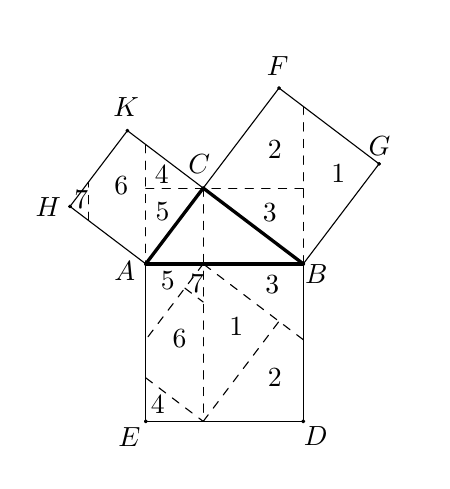
\begin{tikzpicture}[line cap=round,line join=round,>=triangle 45,x=1.0cm,y=1.0cm]
				\clip(-1.5,-2.5) rectangle (3.5,3.);
				\draw [line width=1.2pt] (0.,0.)-- (0.7294706649229483,0.9627117319648537);
				\draw [line width=1.2pt] (0.7294706649229483,0.9627117319648537)-- (2.,0.);
				\draw [line width=1.2pt] (2.,0.)-- (0.,0.);
				\draw [line width=0.4pt] (-0.9627117319648537,0.7294706649229483)-- (0.,0.);
				\draw [line width=0.4pt] (-0.9627117319648537,0.7294706649229483)-- (-0.2332410670419054,1.692182396887802);
				\draw [line width=0.4pt] (-0.2332410670419054,1.692182396887802)-- (0.7294706649229483,0.9627117319648537);
				\draw [line width=0.4pt] (0.7294706649229483,0.9627117319648537)-- (1.692182396887802,2.2332410670419054);
				\draw [line width=0.4pt] (1.692182396887802,2.2332410670419054)-- (2.9627117319648537,1.2705293350770517);
				\draw [line width=0.4pt] (2.9627117319648537,1.2705293350770517)-- (2.,0.);
				\draw [line width=0.4pt] (2.,0.)-- (2.,-2.);
				\draw [line width=0.4pt] (2.,-2.)-- (0.,-2.);
				\draw [line width=0.4pt] (0.,-2.)-- (0.,0.);
				\draw [line width=0.4pt,dash pattern=on 3pt off 3pt] (0.7294706649229483,0.9627117319648537)-- (0.7294706649229483,-2.);
				\draw [line width=0.4pt,dash pattern=on 3pt off 3pt] (0.7294706649229483,-2.)-- (1.692182396887802,-0.7294706649229484);
				\draw [line width=0.4pt,dash pattern=on 3pt off 3pt] (2.,-0.9627117319648537)-- (0.7294706649229483,0.);
				\draw [line width=0.4pt,dash pattern=on 3pt off 3pt] (0.7294706649229483,0.)-- (0.,-0.9627117319648537);
				\draw [line width=0.4pt,dash pattern=on 3pt off 3pt] (0.,-1.447261902691184)-- (0.7294706649229483,-2.);
				\draw [line width=0.4pt,dash pattern=on 3pt off 3pt] (0.,1.51544982927367)-- (0.,0.);
				\draw [line width=0.4pt,dash pattern=on 3pt off 3pt] (2.,0.)-- (2.,2.);
				\draw [line width=0.4pt,dash pattern=on 3pt off 3pt] (2.,0.9627117319648537)-- (0.,0.9627117319648537);
				\draw [line width=0.4pt,dash pattern=on 3pt off 3pt] (-0.7294706649229482,0.5527380973088163)-- (-0.7294706649229482,1.0372882680351465);
				\draw [line width=0.4pt,dash pattern=on 3pt off 3pt] (0.49622959788104276,-0.30781760311219825)-- (0.7294706649229482,-0.4845501707263304);
				\draw (2.2331181822722734,1.378772974186403) node[anchor=north west] {$1$};
				\draw (0.9378903389579959,-0.5557660481996028) node[anchor=north west] {$1$};
				\draw (1.427752151493524,1.6942771924296143) node[anchor=north west] {$2$};
				\draw (1.427752151493524,-1.2116827124420684) node[anchor=north west] {$2$};
				\draw (1.3945411811521322,-0.02439052273735231) node[anchor=north west] {$3$};
				\draw (1.3613302108107406,0.8889111616508908) node[anchor=north west] {$3$};
				\draw (-0.00862231577166849,1.3704702316010553) node[anchor=north west] {$4$};
				\draw (-0.05843877128375609,-1.5437924158559748) node[anchor=north west] {$4$};
				\draw (0.06610236749646291,0.02542593277473368) node[anchor=north west] {$5$};
				\draw (-3.1957318632055656E-4,0.9055166468215862) node[anchor=north west] {$5$};
				\draw (-0.5233923560632404,1.229323607650145) node[anchor=north west] {$6$};
				\draw (0.2155517340327257,-0.7135181573212085) node[anchor=north west] {$6$};
				\draw (-1.0298596537694642,1.054966013357844) node[anchor=north west] {$7$};
				\draw (0.4397257838371199,-0.016087780152004644) node[anchor=north west] {$7$};
				\draw [fill=black] (0.,0.) circle (0.5pt);
				\draw[color=black] (-0.26600733591745446,-0.0866610921274598) node {$A$};
				\draw [fill=black] (2.,0.) circle (0.5pt);
				\draw[color=black] (2.16669624158949,-0.1281748050541981) node {$B$};
				\draw [fill=black] (0.7294706649229483,0.9627117319648537) circle (0.5pt);
				\draw[color=black] (0.68050531881221,1.2666859492842095) node {$C$};
				\draw [fill=black] (2.,-2.) circle (0.5pt);
				\draw[color=black] (2.1583934990041422,-2.187254966220419) node {$D$};
				\draw [fill=black] (1.692182396887802,2.2332410670419054) circle (0.5pt);
				\draw[color=black] (1.6768344290539619,2.5120973370863595) node {$F$};
				\draw [fill=black] (-0.9627117319648537,0.7294706649229483) circle (0.5pt);
				\draw[color=black] (-1.2374282184031626,0.7270076812366113) node {$H$};
				\draw [fill=black] (-0.2332410670419054,1.692182396887802) circle (0.5pt);
				\draw[color=black] (-0.24940185074675858,1.9890245542094565) node {$K$};
				\draw [fill=black] (2.9627117319648537,1.2705293350770517) circle (0.5pt);
				\draw[color=black] (2.968681749997345,1.4908599990885965) node {$G$};
				\draw [fill=black] (0.,-2.) circle (0.5pt);
				\draw[color=black] (-0.20788813782001891,-2.1955577088057665) node {$E$};
			\end{tikzpicture}
		\end{minipage}
		\begin{minipage}{0.48\textwidth}
			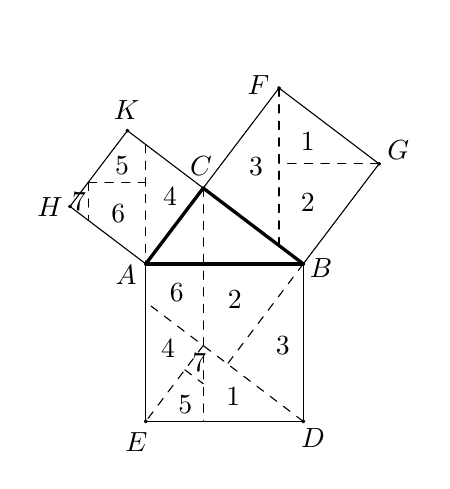
\begin{tikzpicture}[line cap=round,line join=round,>=triangle 45,x=1.0cm,y=1.0cm]
				\clip(-1.5,-2.5) rectangle (3.5,3.);
				\draw [line width=1.2pt] (0.,0.)-- (0.7294706649229483,0.9627117319648537);
				\draw [line width=1.2pt] (0.7294706649229483,0.9627117319648537)-- (2.,0.);
				\draw [line width=1.2pt] (2.,0.)-- (0.,0.);
				\draw [line width=0.4pt] (-0.9627117319648537,0.7294706649229483)-- (0.,0.);
				\draw [line width=0.4pt] (-0.9627117319648537,0.7294706649229483)-- (-0.2332410670419054,1.692182396887802);
				\draw [line width=0.4pt] (-0.2332410670419054,1.692182396887802)-- (0.7294706649229483,0.9627117319648537);
				\draw [line width=0.4pt] (0.7294706649229483,0.9627117319648537)-- (1.692182396887802,2.2332410670419054);
				\draw [line width=0.4pt] (1.692182396887802,2.2332410670419054)-- (2.9627117319648537,1.2705293350770517);
				\draw [line width=0.4pt] (2.9627117319648537,1.2705293350770517)-- (2.,0.);
				\draw [line width=0.4pt] (2.,0.)-- (2.,-2.);
				\draw [line width=0.4pt] (2.,-2.)-- (0.,-2.);
				\draw [line width=0.4pt] (0.,-2.)-- (0.,0.);
				\draw [line width=0.4pt,dash pattern=on 3pt off 3pt] (0.7294706649229483,0.9627117319648537)-- (0.7294706649229483,-2.);
				\draw [line width=0.4pt,dash pattern=on 3pt off 3pt] (2.,-2.)-- (0.,-0.48455017072633005);
				\draw [line width=0.4pt,dash pattern=on 3pt off 3pt] (2.,0.)-- (1.0372882680351463,-1.2705293350770517);
				\draw [line width=0.4pt,dash pattern=on 3pt off 3pt] (1.692182396887802,2.2332410670419054)-- (1.692182396887802,0.23324106704190545);
				\draw [line width=0.4pt,dash pattern=on 3pt off 3pt] (2.9627117319648537,1.2705293350770517)-- (1.692182396887802,1.2705293350770517);
				\draw [line width=0.4pt,dash pattern=on 3pt off 3pt] (0.,1.51544982927367)-- (0.,0.);
				\draw [line width=0.4pt,dash pattern=on 3pt off 3pt] (-0.7294706649229482,1.0372882680351465)-- (0.,1.0372882680351465);
				\draw [line width=0.4pt,dash pattern=on 3pt off 3pt] (-0.7294706649229482,1.0372882680351465)-- (-0.7294706649229482,0.5527380973088163);
				\draw [line width=0.4pt,dash pattern=on 3pt off 3pt] (0.7294706649229482,-1.0372882680351463)-- (0.,-2.);
				\draw [line width=0.4pt,dash pattern=on 3pt off 3pt] (0.49622959788104287,-1.3451058711473443)-- (0.7294706649229482,-1.5218384387614763);
				\draw (1.8462986143761793,1.79107636082032) node[anchor=north west] {$1$};
				\draw (0.8995907295523797,-1.4486626822198103) node[anchor=north west] {$1$};
				\draw (1.8462986143761793,1.0203895400090115) node[anchor=north west] {$2$};
				\draw (0.9186200337699435,-0.21651523413259477) node[anchor=north west] {$2$};
				\draw (1.1897876188702279,1.4723355151761368) node[anchor=north west] {$3$};
				\draw (1.5275577687319855,-0.7969090127682715) node[anchor=north west] {$3$};
				\draw (0.09560262636030888,1.0917494308248734) node[anchor=north west] {$4$};
				\draw (0.07181599608835411,-0.8397249472577887) node[anchor=north west] {$4$};
				\draw (-0.5133351086017329,1.4818501672849185) node[anchor=north west] {$5$};
				\draw (0.2906529945903379,-1.5485665293620168) node[anchor=north west] {$5$};
				\draw (-0.5609083691456425,0.8824270844316785) node[anchor=north west] {$6$};
				\draw (0.18123449533934602,-0.1261260390991697) node[anchor=north west] {$6$};
				\draw (-1.0604276048566925,1.029904192117793) node[anchor=north west] {$7$};
				\draw (0.46667405860280314,-1.0205033373246388) node[anchor=north west] {$7$};					\draw [fill=black] (0.,0.) circle (0.5pt);
				\draw[color=black] (-0.25177832846802064,-0.147630159201721624) node {$A$};
				\draw [fill=black] (2.,0.) circle (0.5pt);
				\draw[color=black] (2.2272693101586153,-0.05372973161414028) node {$B$};
				\draw [fill=black] (0.7294706649229483,0.9627117319648537) circle (0.5pt);
				\draw[color=black] (0.6997830352679597,1.236944028341586) node {$C$};
				\draw [fill=black] (2.,-2.) circle (0.5pt);
				\draw[color=black] (2.1225119841042243,-2.212405819665119) node {$D$};
				\draw [fill=black] (1.692182396887802,2.2332410670419054) circle (0.5pt);
				\draw[color=black] (1.431147509686092,2.274329566772159) node {$F$};
				\draw [fill=black] (-0.9627117319648537,0.7294706649229483) circle (0.5pt);
				\draw[color=black] (-1.2175155175093838,0.7278139876639778) node {$H$};
				\draw [fill=black] (-0.2332410670419054,1.692182396887802) circle (0.5pt);
				\draw[color=black] (-0.24216752350144874,1.9600575886089865) node {$K$};
				\draw [fill=black] (2.9627117319648537,1.2705293350770517) circle (0.5pt);
				\draw[color=black] (3.2078553945098918,1.4469394447393342) node {$G$};
				\draw [fill=black] (0.,-2.) circle (0.5pt);
				\draw[color=black] (-0.11847704608728396,-2.262309666807326) node {$E$};
			\end{tikzpicture}
		\end{minipage}
	\end{figure}
\end{frame}

\begin{frame}
	\begin{figure}
		\centering
		\begin{minipage}{0.48\textwidth}
			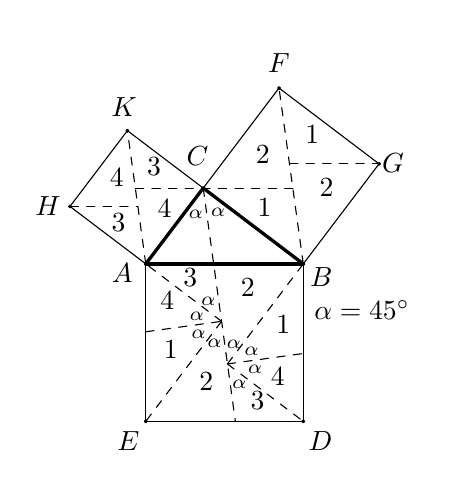
\begin{tikzpicture}[line cap=round,line join=round,>=triangle 45,x=1.0cm,y=1.0cm]
				\clip(-1.5,-2.5) rectangle (3.5,3.);
				\draw [line width=1.2pt] (0.,0.)-- (0.7294706649229483,0.9627117319648537);
				\draw [line width=1.2pt] (0.7294706649229483,0.9627117319648537)-- (2.,0.);
				\draw [line width=1.2pt] (2.,0.)-- (0.,0.);
				\draw [line width=0.4pt] (-0.9627117319648537,0.7294706649229483)-- (0.,0.);
				\draw [line width=0.4pt] (-0.9627117319648537,0.7294706649229483)-- (-0.2332410670419054,1.692182396887802);
				\draw [line width=0.4pt] (-0.2332410670419054,1.692182396887802)-- (0.7294706649229483,0.9627117319648537);
				\draw [line width=0.4pt] (0.7294706649229483,0.9627117319648537)-- (1.692182396887802,2.2332410670419054);
				\draw [line width=0.4pt] (1.692182396887802,2.2332410670419054)-- (2.9627117319648537,1.2705293350770517);
				\draw [line width=0.4pt] (2.9627117319648537,1.2705293350770517)-- (2.,0.);
				\draw [line width=0.4pt] (2.,0.)-- (2.,-2.);
				\draw [line width=0.4pt] (2.,-2.)-- (0.,-2.);
				\draw [line width=0.4pt] (0.,-2.)-- (0.,0.);
				\draw [line width=0.4pt,dash pattern=on 3pt off 3pt] (-0.9627117319648537,0.7294706649229483)-- (-0.1005462038698171,0.7294706649229483);
				\draw [line width=0.4pt,dash pattern=on 3pt off 3pt] (0.,0.)-- (-0.2332410670419054,1.692182396887802);
				\draw [line width=0.4pt,dash pattern=on 3pt off 3pt] (-0.13269486317208828,0.9627117319648537)-- (1.8673051368279117,0.9627117319648537);
				\draw [line width=0.4pt,dash pattern=on 3pt off 3pt] (1.8248772600598901,1.2705293350770517)-- (2.9627117319648537,1.2705293350770517);
				\draw [line width=0.4pt,dash pattern=on 3pt off 3pt] (2.,0.)-- (1.692182396887802,2.2332410670419054);
				\draw [line width=0.4pt,dash pattern=on 3pt off 3pt] (0.7294706649229483,0.9627117319648537)-- (1.1378344719049633,-2.);
				\draw [line width=0.4pt,dash pattern=on 3pt off 3pt] (0.9627117319648536,-0.7294706649229483)-- (0.,-2.);
				\draw [line width=0.4pt,dash pattern=on 3pt off 3pt] (0.,-0.8621655280950367)-- (0.9627117319648536,-0.7294706649229483);
				\draw [line width=0.4pt,dash pattern=on 3pt off 3pt] (0.9627117319648536,-0.7294706649229483)-- (0.,0.);
				\draw [line width=0.4pt,dash pattern=on 3pt off 3pt] (1.037288268035146,-1.2705293350770517)-- (2.,-2.);
				\draw [line width=0.4pt,dash pattern=on 3pt off 3pt] (1.037288268035146,-1.2705293350770517)-- (2.,-1.1378344719049636);
				\draw [line width=0.4pt,dash pattern=on 3pt off 3pt] (1.037288268035146,-1.2705293350770517)-- (2.,0.);
				\draw (0.5778069128004782,-0.3003369658402193) node[anchor=north west] {$\scriptstyle\alpha$};
				\draw (0.7013927076115246,0.8344053319702645) node[anchor=north west] {$\scriptstyle\alpha$};
				\draw (0.4205159012227828,0.8119351874591658) node[anchor=north west] {$\scriptstyle\alpha$};
				\draw (0.4542211179894318,-0.716034639295545) node[anchor=north west] {$\scriptstyle\alpha$};
				\draw (0.43175097347833247,-0.4913331941845581) node[anchor=north west] {$\scriptstyle\alpha$};
				\draw (0.9036240082114186,-0.8396204341065878) node[anchor=north west] {$\scriptstyle\alpha$};
				\draw (0.6564524185893259,-0.8283853618510385) node[anchor=north west] {$\scriptstyle\alpha$};
				\draw (1.1732657423446107,-1.1654375295175188) node[anchor=north west] {$\scriptstyle\alpha$};
				\draw (1.128325453322412,-0.9295010121509826) node[anchor=north west] {$\scriptstyle\alpha$};
				\draw (0.9710344417447166,-1.3564337578618577) node[anchor=north west] {$\scriptstyle\alpha$};
				\draw (2.0170118118107832,-0.34527725486241667) node[anchor=north west] {$\alpha=45^\circ$};
				\draw (1.9035454389553392,1.8792670517363534) node[anchor=north west] {$1$};
				\draw (1.296851537155657,0.9579911267813073) node[anchor=north west] {$1$};
				\draw (1.5327880545222001,-0.5362734832067555) node[anchor=north west] {$1$};
				\draw (0.10593387806739205,-0.8508555063621371) node[anchor=north west] {$1$};
				\draw (1.2743813926445577,1.6208603898587186) node[anchor=north west] {$2$};
				\draw (2.083306595044134,1.205162716403393) node[anchor=north west] {$2$};
				\draw (1.0833851643002135,-0.06440044847368305) node[anchor=north west] {$2$};
				\draw (0.5553367682893788,-1.2553181075619135) node[anchor=north west] {$2$};
				\draw (-0.1075324947880517,1.4748044505365772) node[anchor=north west] {$3$};
				\draw (-0.5569353850100385,0.7669948984369684) node[anchor=north west] {$3$};
				\draw (0.3531054676894848,0.05918534633735973) node[anchor=north west] {$3$};
				\draw (1.2069709591112598,-1.5024896971839992) node[anchor=north west] {$3$};
				\draw (-0.5794055295211379,1.3287485112144357) node[anchor=north west] {$4$};
				\draw (0.02728837227854435,0.9355209822702086) node[anchor=north west] {$4$};
				\draw (0.06099358904519336,-0.23292653230692323) node[anchor=north west] {$4$};
				\draw (1.4653776209889022,-1.1991427462841668) node[anchor=north west] {$4$};
				\draw [fill=black] (0.,0.) circle (0.5pt);
				\draw[color=black] (-0.2985287231323961,-0.11495827362365511) node {$A$};
				\draw [fill=black] (2.,0.) circle (0.5pt);
				\draw[color=black] (2.2293625343662797,-0.17113363490140182) node {$B$};
				\draw [fill=black] (0.7294706649229483,0.9627117319648537) circle (0.5pt);
				\draw[color=black] (0.6564524185893259,1.3680712641088584) node {$C$};
				\draw [fill=black] (2.,-2.) circle (0.5pt);
				\draw[color=black] (2.21812746211073,-2.24962200217803) node {$D$};
				\draw [fill=black] (1.692182396887802,2.2332410670419054) circle (0.5pt);
				\draw[color=black] (1.6900790660998954,2.5477538509415396) node {$F$};
				\draw [fill=black] (-0.9627117319648537,0.7294706649229483) circle (0.5pt);
				\draw[color=black] (-1.2422747925985684,0.7389072177980951) node {$H$};
				\draw [fill=black] (-0.2332410670419054,1.692182396887802) circle (0.5pt);
				\draw[color=black] (-0.27605857862129674,1.9860002381640722) node {$K$};
				\draw [fill=black] (2.9627117319648537,1.2705293350770517) circle (0.5pt);
				\draw[color=black] (3.1394033870658027,1.2781906860644636) node {$G$};
				\draw [fill=black] (0.,-2.) circle (0.5pt);
				\draw[color=black] (-0.21988321734354843,-2.24962200217803) node {$E$};
			\end{tikzpicture}
		\end{minipage}
		\begin{minipage}{0.48\textwidth}
			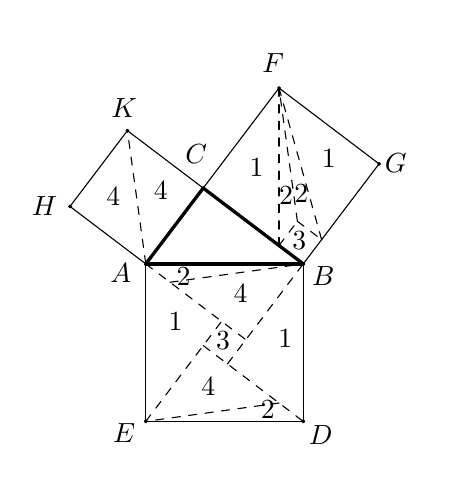
\begin{tikzpicture}[line cap=round,line join=round,>=triangle 45,x=1.0cm,y=1.0cm]
				\clip(-1.5,-2.5) rectangle (3.5,3.);
				\draw [line width=1.2pt] (0.,0.)-- (0.7294706649229483,0.9627117319648537);
				\draw [line width=1.2pt] (0.7294706649229483,0.9627117319648537)-- (2.,0.);
				\draw [line width=1.2pt] (2.,0.)-- (0.,0.);
				\draw [line width=0.4pt] (-0.9627117319648537,0.7294706649229483)-- (0.,0.);
				\draw [line width=0.4pt] (-0.9627117319648537,0.7294706649229483)-- (-0.2332410670419054,1.692182396887802);
				\draw [line width=0.4pt] (-0.2332410670419054,1.692182396887802)-- (0.7294706649229483,0.9627117319648537);
				\draw [line width=0.4pt] (0.7294706649229483,0.9627117319648537)-- (1.692182396887802,2.2332410670419054);
				\draw [line width=0.4pt] (1.692182396887802,2.2332410670419054)-- (2.9627117319648537,1.2705293350770517);
				\draw [line width=0.4pt] (2.9627117319648537,1.2705293350770517)-- (2.,0.);
				\draw [line width=0.4pt] (2.,0.)-- (2.,-2.);
				\draw [line width=0.4pt] (2.,-2.)-- (0.,-2.);
				\draw [line width=0.4pt] (0.,-2.)-- (0.,0.);
				\draw [line width=0.4pt,dash pattern=on 3pt off 3pt] (0.,0.)-- (1.2705293350770517,-0.9627117319648537);
				\draw [line width=0.4pt,dash pattern=on 3pt off 3pt] (1.0372882680351465,-1.2705293350770517)-- (2.,0.);
				\draw [line width=0.4pt,dash pattern=on 3pt off 3pt] (0.7294706649229483,-1.0372882680351463)-- (2.,-2.);
				\draw [line width=0.4pt,dash pattern=on 3pt off 3pt] (0.,-2.)-- (0.9627117319648537,-0.7294706649229482);
				\draw [line width=0.4pt,dash pattern=on 3pt off 3pt] (0.,0.)-- (-0.2332410670419054,1.692182396887802);
				\draw [line width=0.4pt,dash pattern=on 3pt off 3pt] (1.6921823968878018,0.2332410670419054)-- (1.9254234639297074,0.5410586701541032);
				\draw [line width=0.4pt,dash pattern=on 3pt off 3pt] (1.9254234639297074,0.5410586701541032)-- (2.2332410670419054,0.3078176031121979);
				\draw [line width=0.4pt,dash pattern=on 3pt off 3pt] (1.9254234639297074,0.5410586701541032)-- (1.692182396887802,2.2332410670419054);
				\draw [line width=0.4pt,dash pattern=on 3pt off 3pt] (1.692182396887802,2.2332410670419054)-- (1.6921823968878018,0.2332410670419054);
				\draw [line width=0.4pt,dash pattern=on 3pt off 3pt] (2.2332410670419054,0.3078176031121979)-- (1.692182396887802,2.2332410670419054);
				\draw [line width=0.4pt,dash pattern=on 3pt off 3pt] (0.307817603112198,-0.2332410670419054)-- (2.,0.);
				\draw [line width=0.4pt,dash pattern=on 3pt off 3pt] (1.692182396887802,-1.7667589329580946)-- (0.,-2.);
				\draw (1.193810163000057,1.461589066648767) node[anchor=north west] {$1$};
				\draw (2.1115798950262374,1.5720613492074704) node[anchor=north west] {$1$};
				\draw (1.5677163501218343,1.104678615305264) node[anchor=north west] {$2$};
				\draw (1.763167311571854,1.130172218972657) node[anchor=north west] {$2$};
				\draw (1.7376737079044602,0.535321466733485) node[anchor=north west] {$3$};
				\draw (0.7689167685434919,-0.7393587166361693) node[anchor=north west] {$3$};
				\draw (0.9898613336609058,-0.14450796439699728) node[anchor=north west] {$4$};
				\draw (0.5819636749826033,-1.3257116009862102) node[anchor=north west] {$4$};
				\draw (-0.6247335652740414,1.087682879527002) node[anchor=north west] {$4$};
				\draw (-0.02138494514571905,1.164163690529181) node[anchor=north west] {$4$};
				\draw (0.16556814841516956,-0.5014184157405005) node[anchor=north west] {$1$};
				\draw (1.5592184822327029,-0.7053672450796452) node[anchor=north west] {$1$};
				\draw (0.26754256308474517,0.07643660072040945) node[anchor=north west] {$2$};
				\draw (1.338273917115289,-1.6146391092166652) node[anchor=north west] {$2$};
				\draw [fill=black] (0.,0.) circle (0.5pt);
				\draw[color=black] (-0.3188103212653146,-0.11476542678503868) node {$A$};
				\draw [fill=black] (2.,0.) circle (0.5pt);
				\draw[color=black] (2.25604364914147,-0.15725476623069384) node {$B$};
				\draw [fill=black] (0.7294706649229483,0.9627117319648537) circle (0.5pt);
				\draw[color=black] (0.6414487502065225,1.3893571895911534) node {$C$};
				\draw [fill=black] (2.,-2.) circle (0.5pt);
				\draw[color=black] (2.2220521775849447,-2.1797473238438787) node {$D$};
				\draw [fill=black] (1.692182396887802,2.2332410670419054) circle (0.5pt);
				\draw[color=black] (1.618703557456622,2.553565090402104) node {$F$};
				\draw [fill=black] (-0.9627117319648537,0.7294706649229483) circle (0.5pt);
				\draw[color=black] (-1.287567260626283,0.7350213621280641) node {$H$};
				\draw [fill=black] (-0.2332410670419054,1.692182396887802) circle (0.5pt);
				\draw[color=black] (-0.2763209818196581,1.9757100739411944) node {$K$};
				\draw [fill=black] (2.9627117319648537,1.2705293350770517) circle (0.5pt);
				\draw[color=black] (3.1738133811676503,1.27888490703245) node {$G$};
				\draw [fill=black] (0.,-2.) circle (0.5pt);
				\draw[color=black] (-0.2763209818196581,-2.1542537201764858) node {$E$};
			\end{tikzpicture}
		\end{minipage}
	\end{figure}
\end{frame}

\part{}
\begin{frame}
	\begin{center}
		\LARGE\textbf{谢谢大家!}
	\end{center}
\end{frame}
\end{document}